% #############################################################################
% This is Chapter 4
% !TEX root = ../main.tex
% #############################################################################
% Change the Name of the Chapter i the following line
\fancychapter{Evaluation}
%\cleardoublepage
\label{chap:evaluation}
 
The main goal of this dissertation was to study different optimization algorithms capable of handling the computationally complex problems that characterize \ac{BPO}, and to devise strategies for its efficient application to architectural design optimization problems. The goal included both single- and multi-objective optimization. To concretize this study, we proposed and implemented an optimization framework which enabled not only the application of different optimization approaches, but also to use several algorithms within each approach.  Finally, we claimed that the proposed framework allows architects to easily explore automated optimization processes within architectural practices. 

This chapter focuses on the evaluation of the proposed framework from both a qualitative perspective and a quantitative one. In particular, \cref{sec:qualitative} discusses the qualitative properties of the optimization framework, especially, for \ac{BPO} practices, outlining its advantages and disadvantages. On the other hand, \cref{sec:quantitative} tests different optimization algorithms, measuring their adequacy for different \ac{BPO} problems. Moreover, it also appraises the framework in the architectural practice through its application to different \ac{BPO} problems. To this end, we follow the algorithmic framework described in \cref{chap:implement}, which exploits the optimization framework described in \cref{chap:architecture} and the Khepri \ac{AD} tool. 

The evaluation aims to answer the following questions: 
\begin{itemize}
	%\item Do the studied algorithms present benefits for the architectural practice? 
	\item Is there a single algorithm that can consistently, across all case studies, reach the best solution?
	\item Is there any class or subclass of algorithms that constantly outperforms others?
	\item Can any of the algorithms reduce the impact of the expensive simulations typically performed in building design? 
	\item Is the proposed framework tailored for performing optimization in architectural practices? 
	\item How does the proposed framework benefit architectural practices?
\end{itemize}


\section{Qualitative Evaluation}
\label{sec:qualitative}

The qualitative evaluation of optimization frameworks involves considering multiple aspects, including the flexibility, adaptability, diversity of algorithms, ease of use, among others. Calling upon the No Free Luch Theorem (\ac{NFLT}) discussed in \cref{ssec:comparisondfo}, some algorithms are really good solvers for some problems and very poor solvers for others~\cite{Wolpert1997NFLT}. In fact, selecting the right algorithm can have a great impact in the efficiency of optimization processes. Particularly, in building design, to benefit from such performance gains, diversity of algorithms allows to face each problems' characteristics differently, enabling the identification of most promising algorithms. Besides the algorithms' diversity, in order to be easily used by less experienced users, algorithms should be effortlessly run, without the need for many manual changes. Notwithstanding their innate simplicity, optimization frameworks should also be flexible enough to enable more experienced users to fine-tune them, thus fostering more efficient optimization processes. At last, a good framework should adapt to handle different problems.

Regarding the adaptability of the proposed framework, it provides mechanisms to address both single- and multi-objective problems: 15 \ac{SOO} algorithms and 13 \acp{MOEA}, respectively. Simpler approaches, like the design of experiments approach discussed in \cref{ssec:doe}, are also possible using one of the 5 sampling methods available in the framework. Moreover, a core feature of this framework is that it provides 10 \ac{ML} algorithms to be combined with other algorithms, thus  promoting the potential reduction of the time complexity involved in building design. 

Back in \cref{chap:architecture}, we discriminated all the algorithms available in the framework (see \cref{table:algorithms}). When comparing to existing optimization tools in architecture, our solution presents a more extense and diverse set of algorithms, which can be explored to address a wider variety of problems. Moreover, while the existing tools rely on a unique optimization approach, such as \ac{SOO} approaches or Pareto-based optimization ones, the solution hereby proposed supports different approaches.

Unlike competing optimization tools, which are implemented on top of visual programming languages, like Grasshopper and Dynamo, our framework is currently implemented on top of a textual programming language. Although the visual paradigms' graphical feel provides a more comfortable experience to less experienced users, the fact that our framework makes use of the textual paradigm confers more scalability and portability.%, thus allowing users to seamlessly apply optimization to more complex buildings. 
Moreover, to make it more appealing to less experienced users, the developed optimization framework is setup as a ready-to-use tool, where every parameter of the optimization process is configured by default.  

Besides the ready-to-use format, the framework supports detailed configurations of the different algorithms, thus allowing more experienced users to fine-tune and, if desired, to combine different algorithms. 

Moreover, given the importance of testing different algorithms before settling for a single one~\cite{Wortmann2016BBO}, the developed framework provides the necessary mechanisms to facilitate the automated testing of multiple algorithms with no additional efforts for the users. Conversely, competing tools frequently require users' intervention to test different algorithms, either by dragging other optimizer components and making necessary changes in the design script or, when possible, by simply re-configuring the optimization tool to use one of the other supported algorithms. 

Regarding the post-processing and logging mechanisms, the proposed framework is automatically configured to produce complete log files, including all the information about the algorithms and problems being addressed, as well as a real-time log of the different solutions explored during the optimization run. This differs from existing architectural optimization tools, which only produce the log files after the execution. Nevertheless, some of the currently existing optimization tools still visually outperform the developed framework. In fact, while the current framework implementation seldom provides visual interactive Python scripts that read the log files and produce the corresponding plots, some of the existing architectural optimization tools already update the information of the optimization process in real-time. Note, however, that users are also able to visualize a more updated view of the optimization process as long as they re-run the visualization script. 

Finally, in order to use the optimization framework, users only need to create their design's parametric description and to model the corresponding optimization problem, which involves the definition of the variables and its bounds, of the objectives, and, if necessary, of the constraints. In contrast to the existing tools, which require the modification of the optimization script (e.g., drag other components, redefine the optimization problem, change the optimization tool), our framework requires no such efforts to use different algorithms and/or optimization approaches. Instead, users are only required to specify the algorithms that they wish to apply and to configure them accordingly.

\todo{Tabela sumarizar avaliação S:}

% #############################################################################
\section{Quantitative Evaluation}
\label{sec:quantitative}

In order to study and explore the effectiveness of algorithms within building design practices, we evaluated the performance of different algorithms using the optimization framework, discussed in \cref{chap:implement}. Moreover, we evaluated the real applicability of such framework in three case studies, two of which were proposed by an architectural studio\footnote{Atelier dos Remédios: http://atrem.eu/}: (1) the optimization of the lighting conditions of a solarium in a private house in Portugal; (2) the optimization of the structural behavior and elegance of an arc-shaped space frame structure; and (3) the optimization of the cost and the lighting conditions of an exhibition room in an urban museum.   

In order to measure the effectiveness of the optimization algorithms, different factors must be considered: (1) the optimization time is sensitive to the computational power of the machine where the algorithm is being run, (2) the non-determinism of several optimization algorithms, and (3) the hyperparameters of optimization algorithms. Firstly, to remove the time dependency of the machine characteristics and objective function's complexity, we measure the performance of the optimization algorithm in terms of the number of function evaluations, which is proportional to the actual time spent by the optimization process. Secondly, the stochastic character of several optimization algorithms (e.g., random modifications of solutions, random generation of design solutions, random initial points) might yield different results even when ran twice under the same configurations. To address this limitation, we run each stochastic algorithm three times and we use the average of the values to draw conclusions. Finally, an algorithm's performance for each problem can be better or worse depending on its configurations. To this end, we opt for using the default algorithm's configurations, thus emulating the case when the architect's knowledge does not suffice to properly fine-tune the algorithm. 

\todo{ESCLARECER diferença entre combined PFs, true PFs, Approximated PFs}
% #############################################################################
\subsection{Ericeira House: Solarium}
The first \ac{BPO} case study involved the optimization of the daylight conditions of a room in an isolated private house in Portugal~\cite{Caetano2018,Belem2018optimizeddesign}. The room was designed with a set of façade shading panels that modulate the daylight conditions on the interior of the room. Depicted in \cref{fig:ericeira_panels_explanation}, the panels are composed of a set of horizontal wood bars of different sizes, which alternate between one full-length bar and a set of smaller bars. For aesthetics reasons, the size and position of the smaller bars along the panel's width were randomized. The final pattern of the façade's shading panels was defined in terms of the length’s step, the maximum distance separating two consecutive bars, and the minimum and maximum lengths of the smaller bars. Initially, the goal was to find a solution for the shading panels that maximized the room's daylight performance, which was measured using the \ac{sUDI} metric~\cite{Nabil2006}. While, in general, it is known that the more openings in the shading panels, the more daylight enter the room, this may also cause situations of uncomfortable glare. As a result, these situations should be accounted for, and, notwithstanding the values of the optimization process, architects should always perceive optimization results with a critical thinking. \Cref{fig:ericeira_multiple_panels} represents some design variations, ranging from denser patterns, with lower \ac{sUDI} values, to sparser ones, with higher \ac{sUDI} values.

\begin{figure}[htbp]
	\centering
	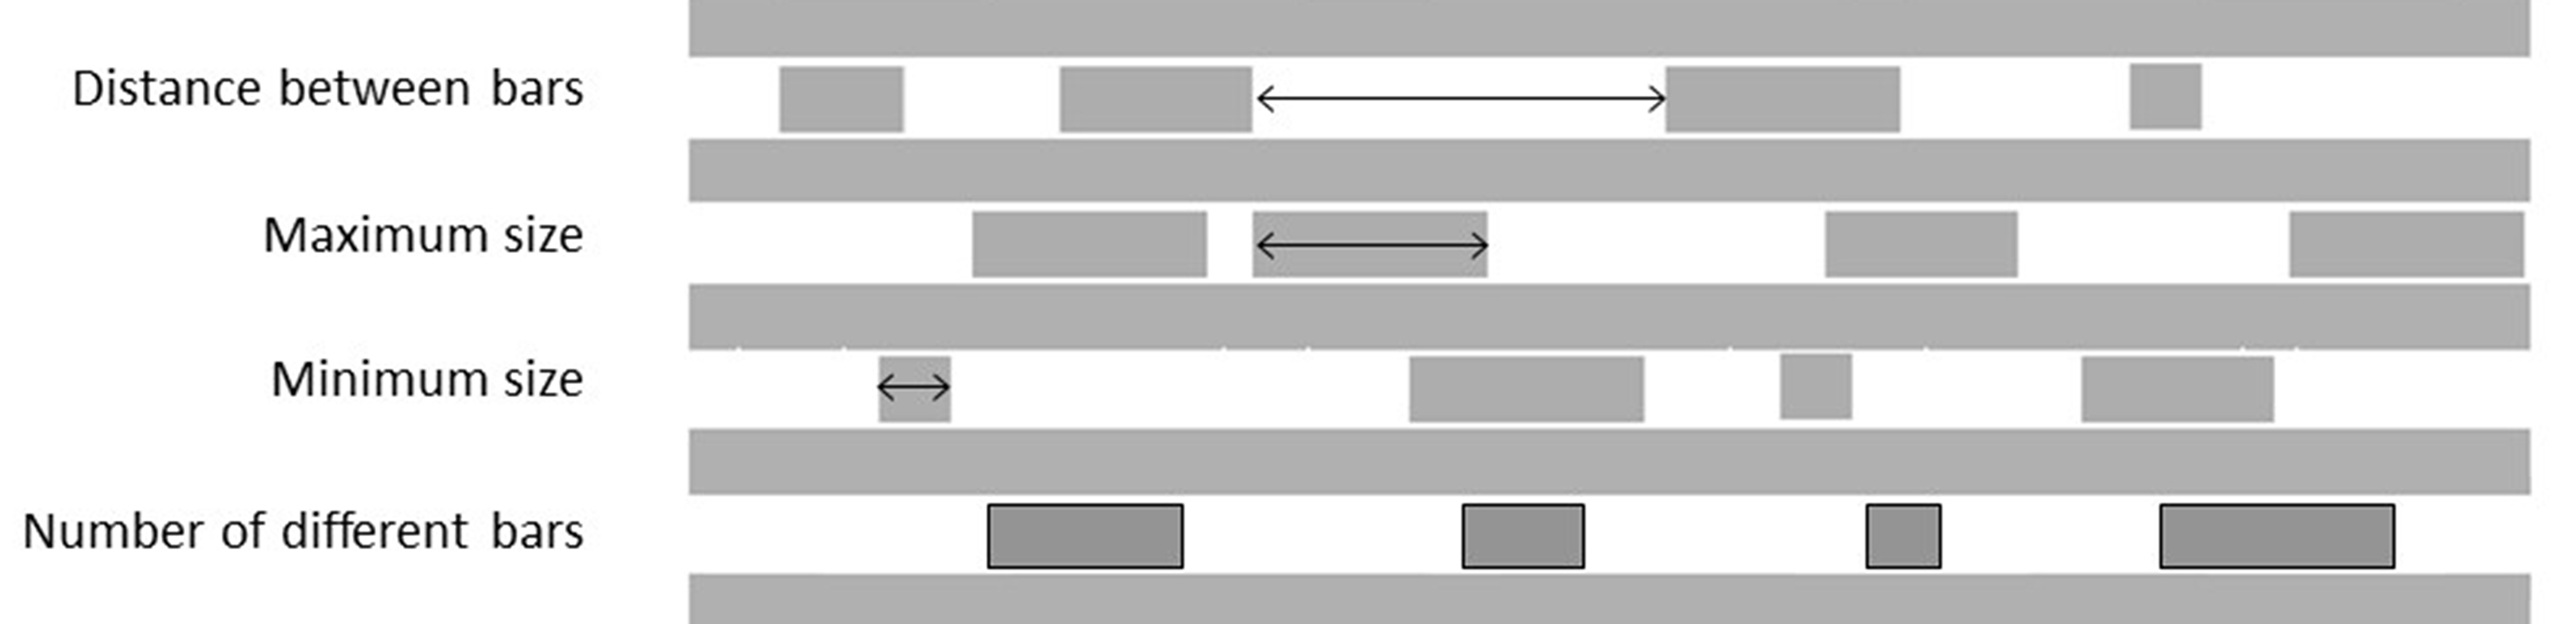
\includegraphics[width=\textwidth]{Images/Evaluation/Ericeira_1.jpg}
	\caption{Ericeira Solarium: Representation of the shading panels' geometric pattern and design variables.}
	\label{fig:ericeira_panels_explanation}
\end{figure}

\begin{figure}
	\centering
	\includegraphics[width=\textwidth]{Images/Evaluation/Ericeira_2.png}
	\caption{Ericeira Solarium: Representation of the shading panels’ geometric pattern with different sUDI values (from left to right, 7\%, 62\%, 90\%, and 100\%).}
	\label{fig:ericeira_multiple_panels}
\end{figure}

Initially, we pursued a simple design of experiments approach to address this optimization problem \cite{Caetano2018}. To generate the design variants to evaluate, we used the random (or Monte Carlo) and the latin hypercube sampling algorithms (see \cref{appendix:AlgorithmsDefinitions}). Following such approach allowed us to exploit previous knowledge about the shading panels and its impact on the daylight conditions of the room (e.g., that sparser patterns increase daylight performance) and, consequently, to produce a more efficient optimization process. In fact, based on this knowledge, we set several iterations of the different sampling methods and, within each iteration, we have further restrained the variables' to vary in smaller ranges, thus enforcing the sampling of incrementally more efficient designs. %\Cref{fig:ericeira_doe} shows an example of the results obtained during this process, as well as the solutions that were presented to the architects, so that they would choose the one that better suited their intentions.

%\begin{figure}[htbp]
%	\centering
%	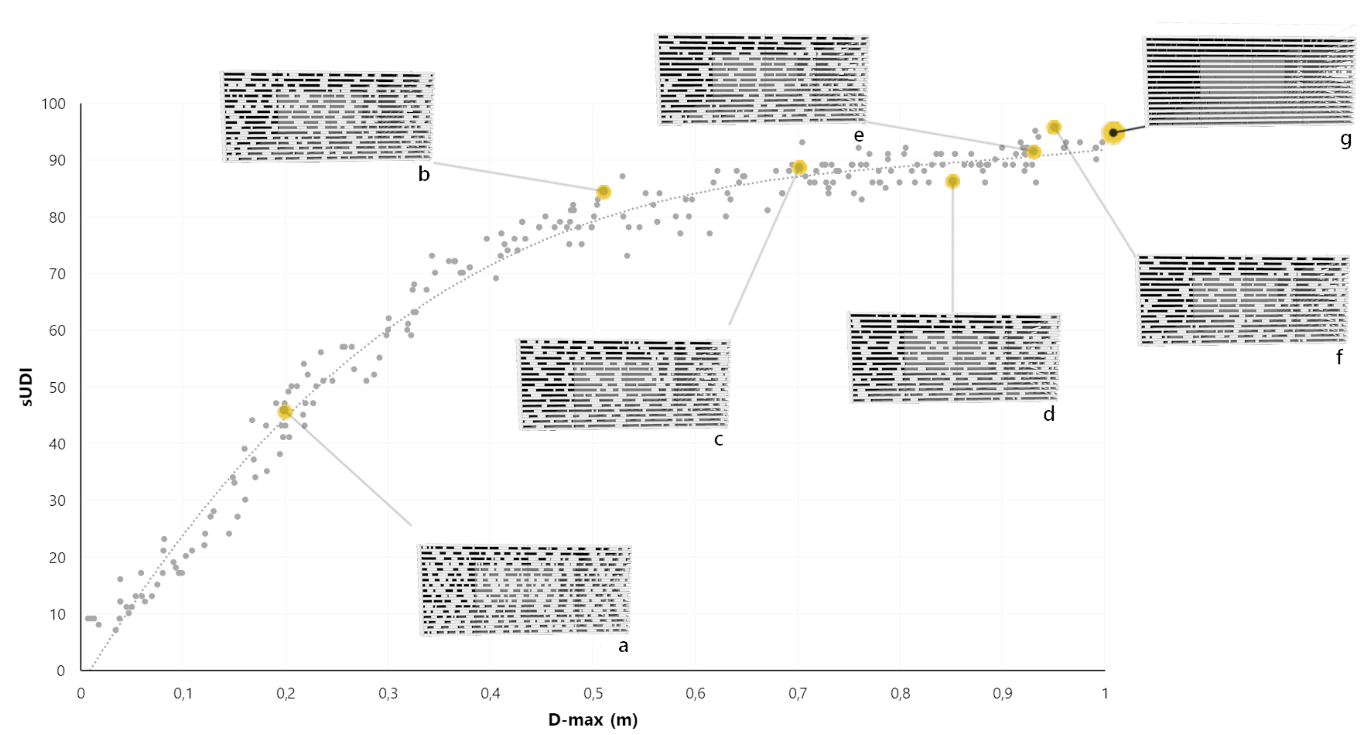
\includegraphics[width=\textwidth]{Images/Evaluation/Ericeira_caadria2018.PNG}
%	\caption{Ericeira Solarium: The scatter plot with the samples obtained during the design of experiments approach. The models a. to g. correspond to the set of examples presented to the architects.}
%	\label{fig:ericeira_doe}
%\end{figure}

Despite achieving optimal solutions with values of sUDI of $100\%$, we have only achieved these solutions after 200 function evaluations. Because each evaluation took approximately $7$ minutes to complete on dual \textit{Intel Xeon CPU E5-2670 @ 2.60GHz, 64GB RAM}, the optimal solution was only obtained after $1400$ minutes, or, equivalently, $23.33$ hours. This large time complexity resulted from the fact that approaches based on sampling algorithms consist on the consecutive uniformed experimentation of multiple designs, i.e., without taking into consideration previous design evaluations, often evaluating irrelevant design solutions. Moreover, this approach required several manual interventions (e.g., analyse the results, redefine the variables' bounds, select number of evaluations). In an attempt to minimize the time complexity of the optimization process and to verify the impact of more guided approaches in \ac{BPO} problems, we have also approached this problem using a \ac{SOO} approach \cite{Belem2018optimizeddesign}. Particularly, we evaluated the performance of $13$ different derivative-free optimization algorithms: $5$ direct-search, $3$ metaheuristics, and $5$ model-based. Given the time complexity of each function evaluation, we set a limit of $60$ function evaluations per run.

%http://papers.cumincad.org/data/works/att/caadria2018\_278.pdf
\begin{table}[htbp]
	\centering
	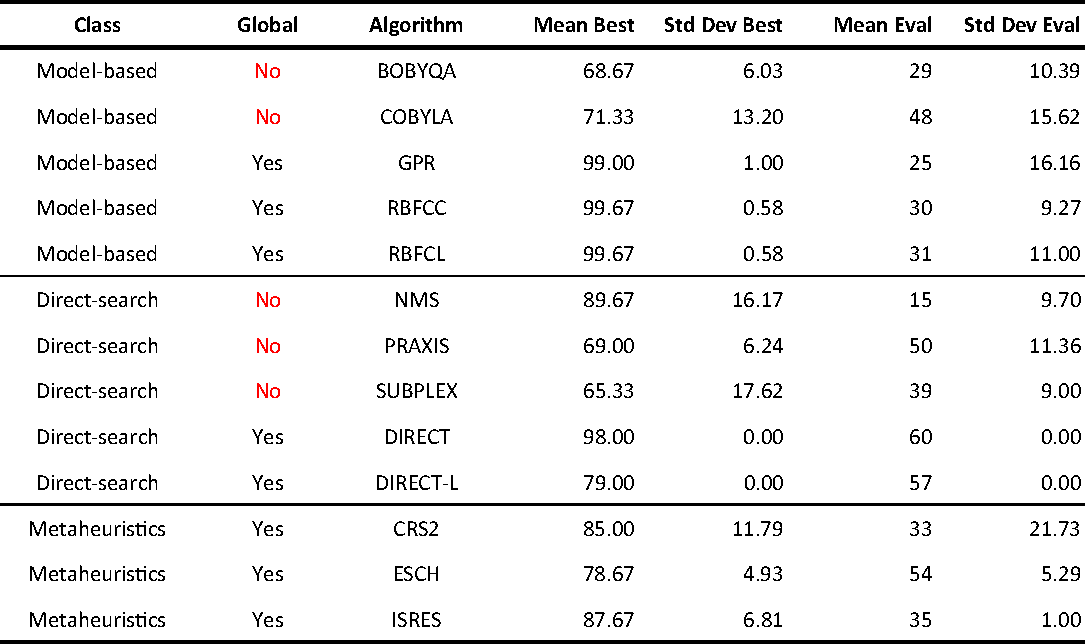
\includegraphics[width=0.8\textwidth]{tables_and_code/Ericeira_phase1_stats_v1.pdf}
	\caption[Ericeira Solarium: Mean best results and evaluations discriminated per algorithm]{Ericeira Solarium: Table with the mean best daylight results and mean evaluations to reach optimal solutions of each algorithm. Results are averaged over $3$ runs, each with $60$ evaluations.}
	\label{table:phase1results}
\end{table}

\Cref{table:phase1results} shows the mean best results and the standard deviation of the $3$ runs,  discriminated by algorithm. According to the results, in average, the global model-based algorithms $GPR$, $RBFCC$, and $RBFCL$ were able to find an optimal solution within the first $30$ evaluations. Conversely, the local model-based algorithms $COBYLA$ and $BOBYQA$ performed rather poorly in this problem, converging to far from optimal solutions after $29$ and $48$ function evaluations, respectively. Regarding direct-search algorithms, the global algorithm $DIRECT$ was able to find a close to optimal solution (with an \ac{sUDI} value of $98\%$) in the last function evaluation. Its local variant, $DIRECT$-$L$, and the local direct-search algorithms $PRAXIS$ and $SUBPLEX$ fell short of the expected and barely managed to improve over $80\%$. Nevertheless, the simplex-based direct-search algorithm $NMS$ performed surprisingly well, having achieved an average result of $89.67\%$ within the first $15$ evaluations. Finally, although metaheuristics performed better than most local model-based and direct-search algorithms, they seem to stagnate in design solutions with \ac{sUDI} values below the $88\%$, after $30$ evaluations.

\Cref{fig:phase1results} shows the average performance per algorithm class, also separating them in local or global algorithms. Overall, local algorithms seem to perform worse than all other algorithms, with local direct-search and model-based algorithms stagnating towards design solutions with \ac{sUDI} values below $75\%$ and $70\%$, respectively. Contrastingly, global algorithms were able to find design solutions with values of \ac{sUDI} larger than $80\%$. Despite the good initial performance of metaheuristics algorithms for the first $20$ evaluations, global direct-search algorithms quickly surpassed them, achieving close to optimal solutions with \ac{sUDI} values of $90\%$. Lastly, global model-based algorithms were, on average, the best performing algorithms, achieving close to optimal solutions shortly after $24$ evaluations. 

\begin{figure}[htbp]
	\centering
	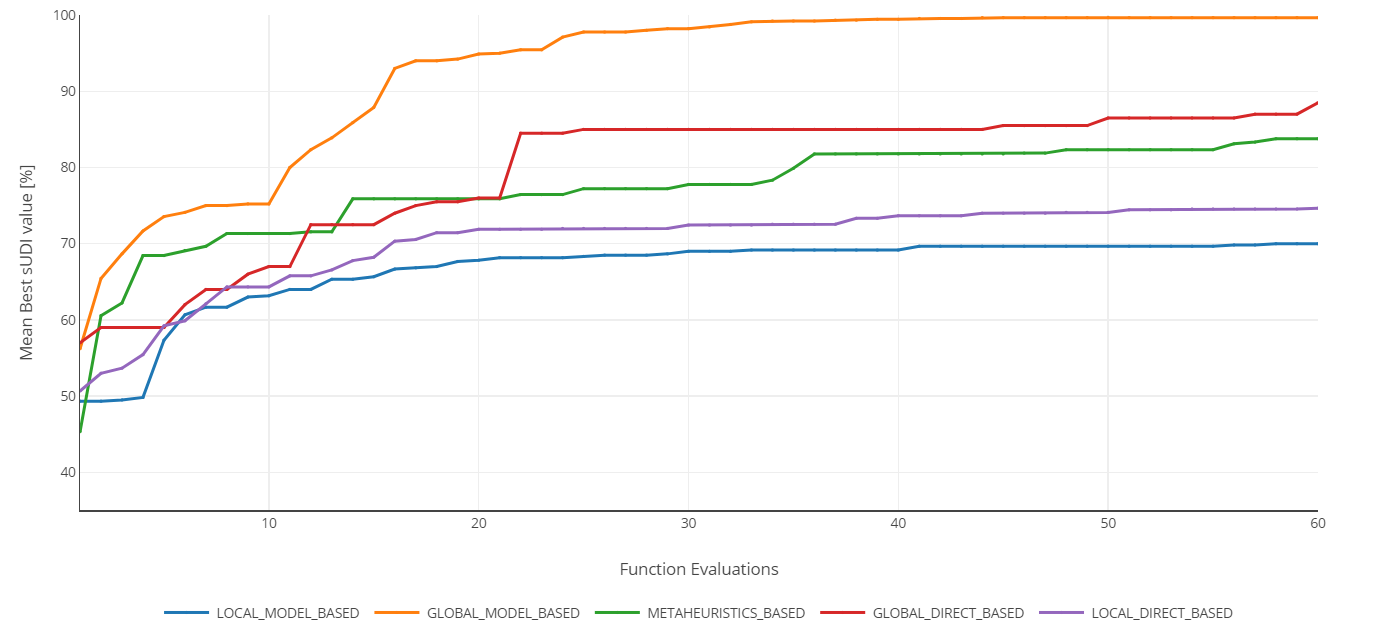
\includegraphics[width=1\textwidth]{Images/Evaluation/Ericeira_results_ph1_per_class.PNG}
	\caption[Ericeira Solarium: Mean best daylight results in function of the number of evaluations, discriminated per class of algorithms]{Ericeira Solarium: Mean best daylight results in function of the number of evaluations, discriminated per class of algorithms.}
	\label{fig:phase1results}
\end{figure}

Given the overall bad performance of local algorithms, we decided to assess their performance when submitted to different initial solutions. Notwithstanding their ability to quickly converge to locally optimal solutions, the quality of the found solutions highly depends on the solution used to initialize the search. As a consequence, we have also studied the impact of different initial solutions in the performance of these algorithms. To this end, we tested all $5$ local algorithms with two different initial solutions: a bad solution, with a $7\%$ value of \ac{sUDI}, and a reasonable solution with a $78\%$ value of \ac{sUDI}. Moreover, we decided to further restrict the number of evaluations to $15$, thus emulating an hypothetical scenario, where users lack knowledge about different optimization algorithms and, as a consequence, opt for testing several algorithms. Ideally, this test would allow them to infer the most promising algorithm and obtain a reasonable solution to hot-start other algorithms and, potentially, improve the overall optimization time.

\Cref{fig:phase2results} presents the mean best daylight results found by each local optimization algorithm. As expected, no local algorithm was able to obtain a good solution when provided with a bad starting solution. On the one hand, when provided with a mild initial design, both $COBYLA$ and $NMS$ found the best designs achieving a \ac{sUDI} value of $99\%$. On the contrary, $PRAXIS$ found the worse, and showed no relevant improvement over the initial design in terms of daylight illuminance. Nevertheless, it initially managed to outperform other methods, achieving values of \ac{sUDI} of $80\%$. After $8$ evaluations, $COBYLA$ and $NMS$ quickly converged to near optimal designs, with \ac{sUDI} values of $99\%$ and $98\%$, respectively. $BOBYQA$ and $SUBPLEX$ struggled to improve from the initial design.

On the other hand, when provided with a bad initial design, the best daylight result has an \ac{sUDI} value of $15\%$ and was found by $NMS$ after $9$ evaluations. $NMS$, $COBYLA$, and $SUBPLEX$ exhibit similar performance, stagnating in a design with an \ac{sUDI} value of $11\%$ after $3$ evaluations, with $NMS$ being able to further improve the design after $5$ evaluations. $PRAXIS$ exhibits the worst performance among all methods, showing no significant improvements throughout the whole optimization process.

\begin{figure}[htbp]
	\centering
	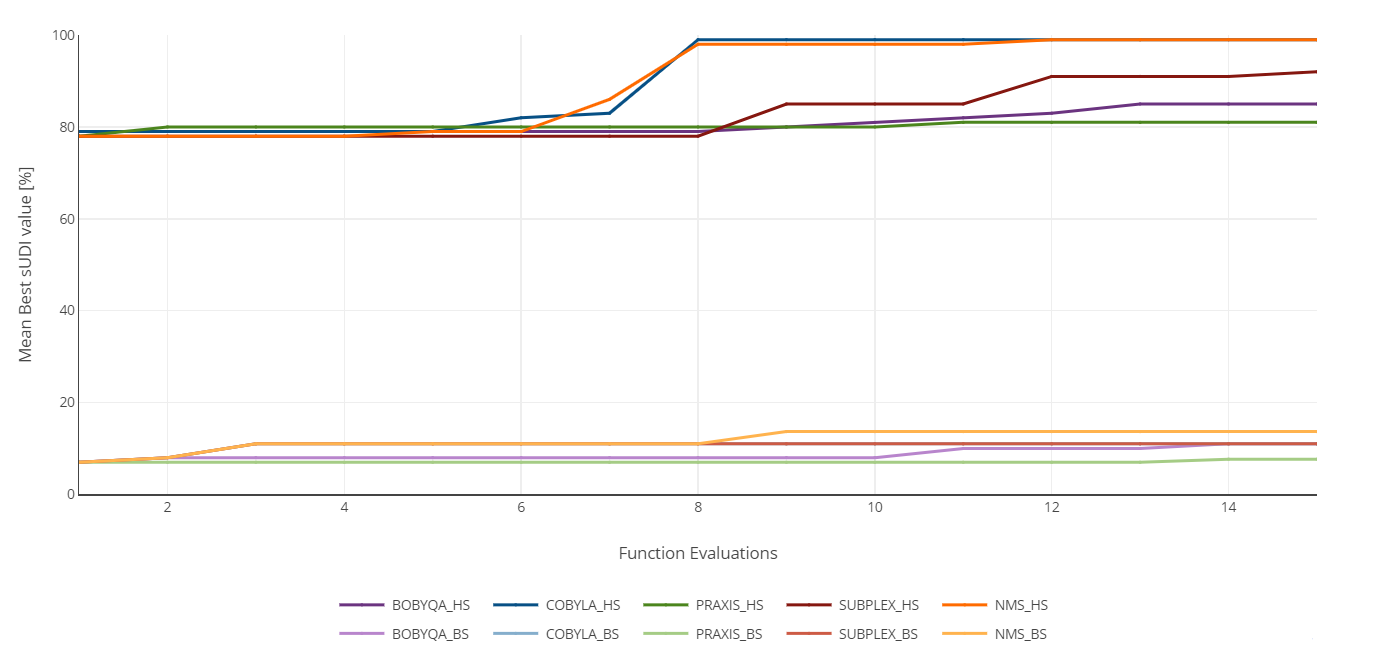
\includegraphics[width=\textwidth]{Images/Evaluation/Ericeira_results_ph2.PNG}
	\caption[Ericeira Solarium: Mean best results of daylight performance in function of the number of evaluations, discriminated per local algorithm]{Ericeira Solarium: Mean best results daylight results as a function of the number of function evaluations, discriminated per local algorithm. Algorithms suffixed with $HS$ are given an initial solution with an \ac{sUDI} value of $78\%$, whilst algorithms suffixed with $BS$ are given an initial solution with an \ac{sUDI} value of $7\%$.}
	\label{fig:phase2results}
\end{figure}


% #############################################################################
\subsection{Space Frame Optimization}

In this section, we address the first of two \ac{MOO} problems \cite{Belem2019MOO,IP2019MOO}. Motivated by the interest of architects in performing structural analysis \cite{Cichocka2017SURVEY}, the first case consisted in the optimization of both the structural behavior and an \textit{ad-hoc} measure of irregularity of an arc-shaped space frame. To instil irregularities in this space frame, we introduced three attractors that cause a deformation in the shape of the truss, each of which is defined in terms of its fixed-radius cylindrical coordinates in the arc-shaped space frame~\cite{Belem2019MOO}. To measure the goals for each design variant, we used (1) the Robot analysis tool to compute the maximum displacement of the structure, and (2) the sum of the Euclidean distances between the attractors. To increase the interest of this case study, we set out to minimize both objectives, thus promoting the conflict between them: placing the attractors near each other will weaken the structure and, thus, the maximum displacement of the space frame. In fact, to reduce the maximum displacement, the attractors should be scattered across the space frame but this implies larger distances among the three attractors and, thus, a less interesting shape. \Cref{fig:spaceframe} illustrates three examples of the space frame structure. 

\begin{figure}[htbp]
	\centering
	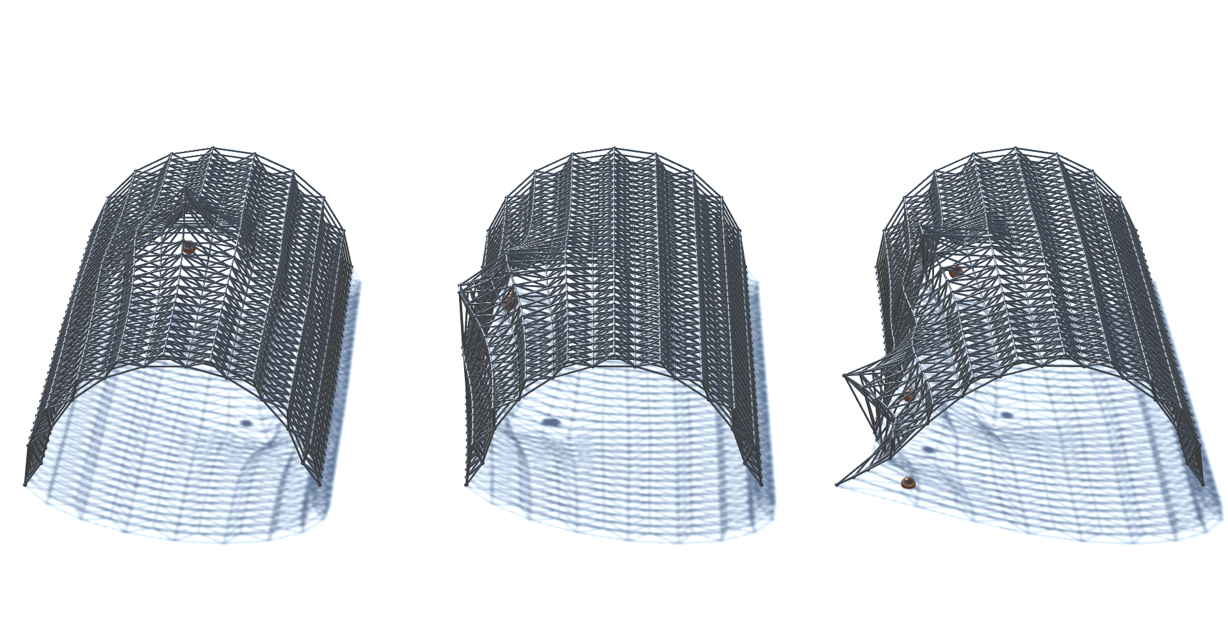
\includegraphics[width=1\textwidth]{Images/Evaluation/truss-kat.png}
	\caption[Space Frame: Representation of three space frame design variants]{Space Frame: Representation of three design variations of the arc-shaped space frame, with copper balls representing the three attractors.}
	\label{fig:spaceframe}
\end{figure}

To optimize the space frame, we decided to test $10$ metaheuristics and $9$ model-based algorithms. On the one hand, each metaheuristic algorithm comprised a total of $15$ individuals/particles per iteration, which were evolved for $15$ iterations. On the other hand, model-based algorithms derived $100$ initial samples using the latin hypercube sampling algorithm, which were then used to create the initial approximation to the expensive evaluation function, upon which another $125$ evaluations were completed. Overall, every algorithm was limited to a total of $225$ function evaluations, each taking approximately $40$ seconds to complete on dual \textit{Intel Xeon CPU E5-2670 @ 2.60GHz, 64GB RAM}. 

The evaluation of these algorithms consisted in the computation of different unary performance indicators discussed in \cref{ssec:performance}, some of which required a reference set to be compared with. Ideally, this reference set would represent the true Pareto front in order to obtain a more fine-grained measure of each algorithm's performance. However this is not possible and, to better approximate the true Pareto front, we determined for each run the set of optimal solutions, which we named the combined Pareto front. Each run is composed of $4275$ candidate solutions. Afterwards, in an attempt to measure the average performance of each algorithm, we computed several performance indicators for each run, using as reference set the combined Pareto front of each run. Although this does not represent an accurate approximation to true Pareto front, we aim at measuring the average performance of each algorithm. To overcome this limitation, the algorithms should be allowed to run for thousands of iterations instead of a few hundreds. Unfortunately, time is frequently a limiting factor in \ac{BPO} problems, and, as a consequence, in the absence of the information about the true Pareto front, we have adopted a methodology similar to the one used for \ac{SOO}, which quantifies the performance of each algorithm in terms of the average of the different runs. 

\Cref{table:spaceframe,table:spaceframestd} show the mean results of the performance indicators and corresponding standard deviations for the three runs, discriminated by class and subclass. Since we are addressing a \ac{MOO} problem, we measured the each algorithm's results in terms of several performance indicators. These indicators provide information about the three different relevant aspects of Pareto fronts: (1) the cardinality, measured by \ac{ONVG}, \ac{ONVGR}, and \ac{ER}; (2) the diversity, measured with Spacing and Maximum Spread; and (3) accuracy/convergence, measured with \ac{MPFE} and \ac{GD}. Moreover, we use two additional indicators, \ac{HV} and \ac{IGD}, to obtain a combined measure of all the three aspects mentioned. % To simplify the performance comparison among the different algorithms, we restrained the set of indicators to the unary ones. 
% 1 - Two set coverage não ia dar medidas relevantes porque raramente as diferentes frentes se tocam. 
% 2 - Epsilon indicators poderia ser interessante, mas não foi testada a implementação
% 3 - R-metrics requer funções de utilidade que não temos e que requer alguma sensibilidade em relação ao problema...

% The overall cardinality of each combined Pareto front is 14, 24, and 19, respectively.
When considering the cardinality aspect, metaheuristics seem to retrieve the most nondominated solutions within each run, whereas the model-based algorithms seem to retrieve the least. In fact, among the model-based algorithms, the algorithms exploring random search strategies, i.e., the algorithms suffixed with $Random$, yield fewer nondominated solutions, which may result from a poor exploration of the solution space. This tendency is further translated when we compare the optimal solutions ratio between each algorithm and the combined Pareto fronts. The \ac{ONVGR} column of \cref{table:spaceframe} presents this ratio. On average, $PAES$ is able to find twice the number of solutions that compose each combined Pareto front, whereas model-based algorithms, including $GPR$+$Random$ and \acp{MLP} algorithms struggled to find a set of optimal solutions with at least half of the size of the combined Pareto fronts. 

%http://papers.cumincad.org/data/works/att/caadria2018\_278.pdf
\begin{table}[h!]
	\centering
	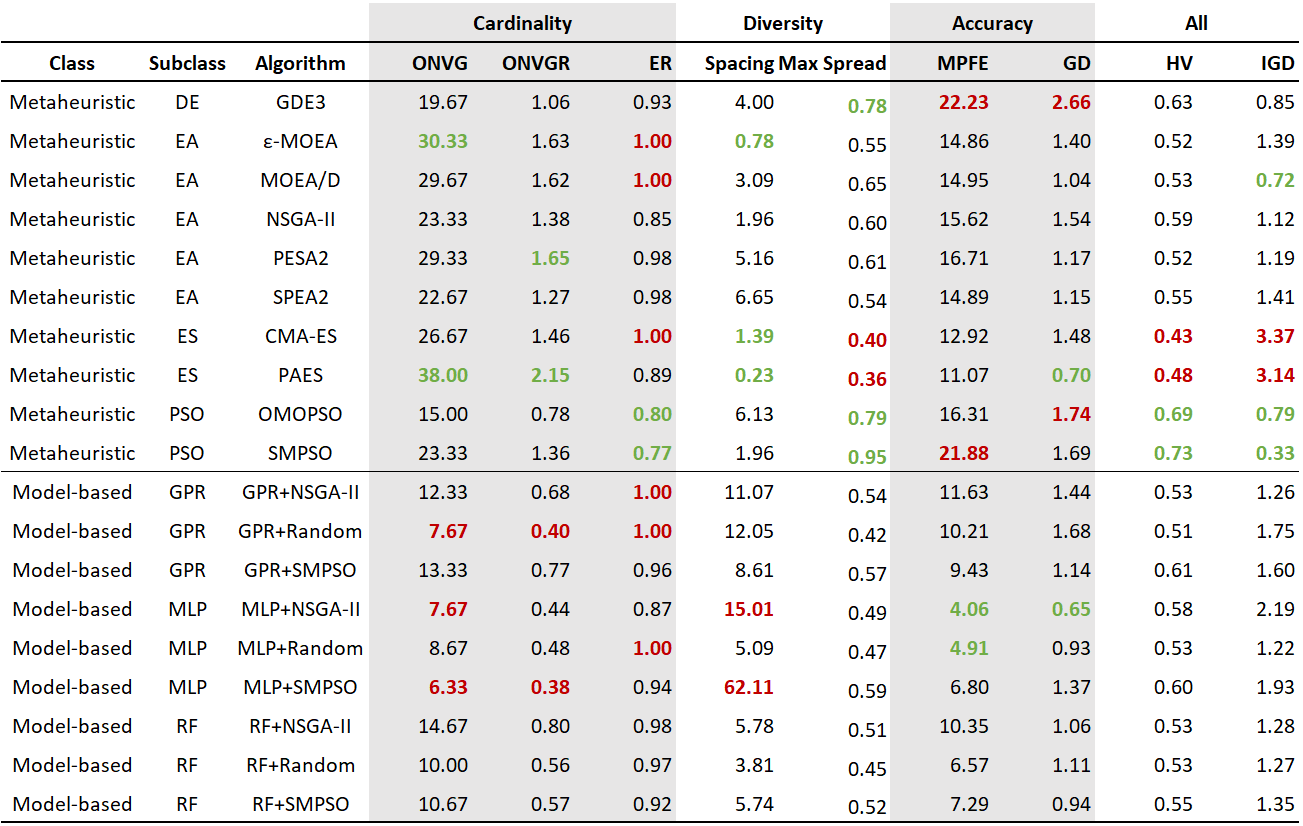
\includegraphics[width=\textwidth]{Images/Evaluation/caadria/Results_Mean_20190416.PNG}
	\caption[Space Frame: Mean results of each algorithm, measured in terms of unary MOO performance indicators, discriminated per algorithms]{Space Frame: Comparison of the algorithms' mean results for the bi-objective space frame optimization problem. Results are averaged over $3$ runs, each with $225$ evaluations.}
	\label{table:spaceframe}
\end{table}

While \ac{ONVG} and \ac{ONVGR} indicators provide an intuition about the richness of the algorithms' Pareto fronts, many of the identified solutions might not be truly optimal, i.e., despite being optimal among all the evaluated solutions, these solutions might not belong to the true Pareto front or, in this case, to the combined Pareto front of the corresponding run. To this end, \ac{ER} is used to measure the percentage of false-optimal solutions for each algorithm. In this case, it becomes clear that even though $PAES$ retrieves twice as many optimal solutions as the combined fronts, most of them are not truly optimal. Moreover, none of the solutions found by the $\epsilon$-$MOEA$, $MOEA$/$D$, and $CMA$-$ES$ metaheuristics algorithms belong to the combined front. The same happens with some of the model-based algorithms, particularly, $GPR$+$NSGA$-$II$, $GPR$+$Random$, and $MLP$+$Random$. On the other hand, \ac{PSO}-based metaheuristics algorithms, $SMPSO$ and $OMOPSO$, exhibit the lowest \ac{ER} value, having found at least one true optimal solution in each run (see \cref{appendix:appendixB} for a more detailed view over the results of the three runs).

The diversity aspect consists in the analysis of the distribution of the nondominated solutions across the objective space. The Spacing indicator measures the uniformity of the set of optimal solutions retrieved by each algorithm, regardless of the combined Pareto front. Considering this indicator, the two \ac{ES}-based metaheuristic algorithms, $PAES$ and $CMA$-$ES$, and one \ac{EA}-based metaheuristic algorithm, $\epsilon$-$MOEA$, achieved the most uniform Pareto fronts. Conversely, model-based algorithms seem to yield more irregular Pareto fronts, namely, $MLP+NSGA-II$ and $MLP+SMPSO$ achieved the worst values of the Spacing indicator. Note, however, that this indicator merely provides an idea of the regularity of distribution of the solutions. Ideally, this indicator would also suggest a good coverage of the combined Pareto front, i.e., that the Pareto front found by each algorithm covers the same regions as the combined Pareto front, instead of focusing on a single smaller region. However, most of the algorithms which present the best scores in the Spacing indicator achieve such values because most of the identified optimal solutions lie within the same small region in the solution space, thus yielding a more uniform distribution. Additionally, these indicators are highly sensitive to outliers and to the number of retrieved solutions. % number of solutions also indirectly contributes to these scores of each indicators, since these indicators measure the distances between consecutive optimal solutions and the weight each outlier has in smaller or larger sets can greatly influence the final result.

Besides having an uniform distribution, when applicable, a good Pareto front should also cover large extents of the objective space in order to provide more relevant trade-offs. The Maximum Spread indicator (named Max Spread in \cref{table:spaceframe,table:spaceframestd}) measures the extent of the Pareto fronts retrieved by each algorithm. On average, $SMPSO$, $GDE3$, and $OMOPSO$ are able to explore wider extents of the solution space. Observing \cref{table:spaceframe}, we conclude that, on average, $SMPSO$, $GDE3$, and $OMOPSO$ were able to cover the objective space better. Constrastingly, the \ac{ES}-based algorithms were the worst algorithms in this aspect, having explored smaller regions of the objective space. Regarding model-based algorithms, it is possible to observe that the ones based on $SMPSO$ were able to explore broader regions of the objective space than the ones based on $NSGA$-$II$ or $Random$ strategies. 

\begin{table}[h!]
	\centering
	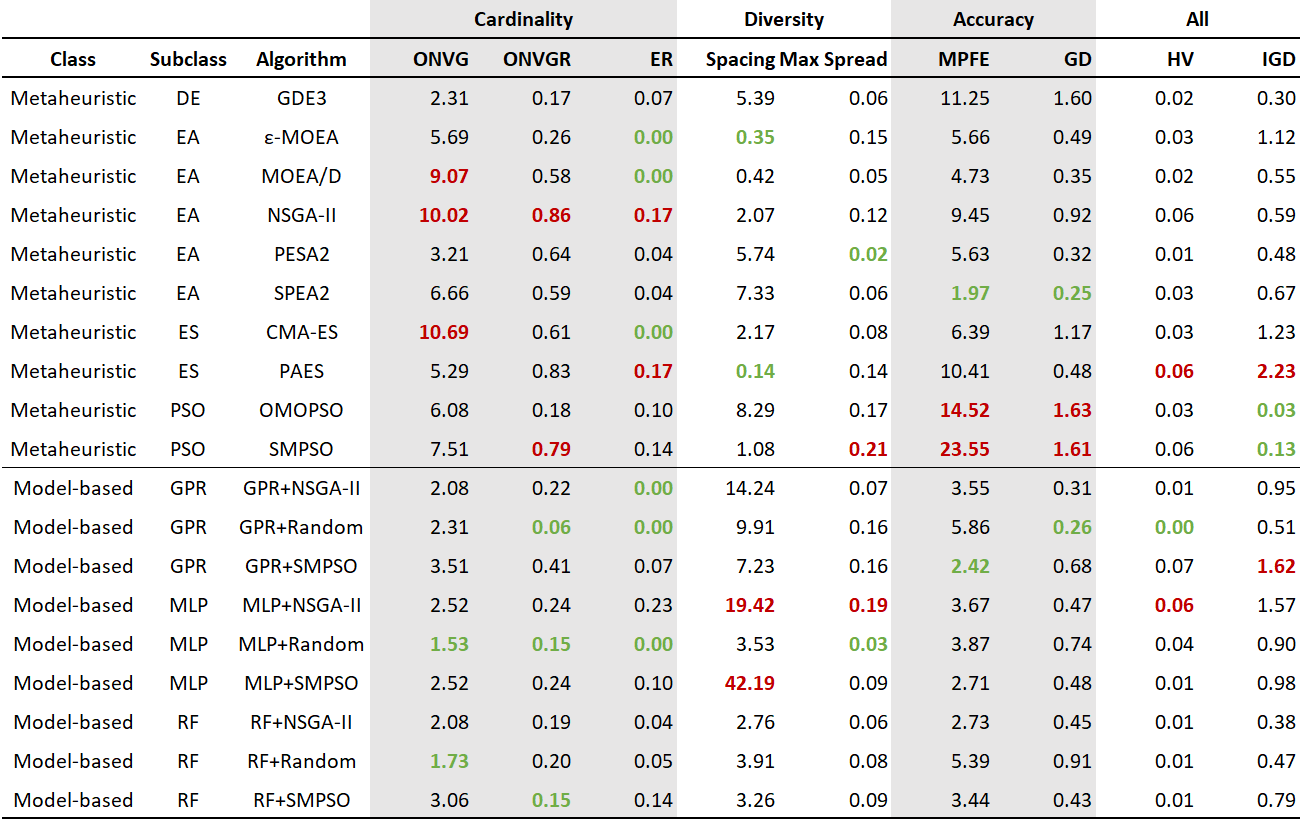
\includegraphics[width=\textwidth]{Images/Evaluation/caadria/Results_Std_20190416.PNG}
	\caption[Space Frame: Standard deviations of the performance indicators results, discriminated by each algorithm]{Space Frame: Standard deviation values for the performance indicators, discriminated by algorithm. Results are averaged over $3$ runs, each with $225$ evaluations.}
	\label{table:spaceframestd}
\end{table}

Another important aspect of Pareto fronts is their accuracy and how close their solutions are from the true Pareto front. As previously mentioned, in this dissertation, we consider the true Pareto front to be the result of the best solutions found in each run. This decision aims at measuring the average performance of each algorithm even when the real true Pareto front is unknown. In this case study, we used two accuracy indicators, \ac{MPFE} and \ac{GD}. On average, when considering \ac{MPFE}, every model-based algorithm retrieved Pareto fronts, whose \ac{MPFE} values were always better than the ones obtained by any metaheuristic. In particular, $MLP$+$NSGA$-$II$ and $MLP$+$Random$ have the smallest maximum error which means that all the points are at most at that distance from an optimal solution. Furthermore, the algorithms exploring a larger extent of the objective space, i.e., with higher values of Max Spread, have worse \ac{MPFE} values. This can be explained due to the lack of information about the true Pareto front, which is only approximated by the best solutions found in each run. 

Notwithstanding the fact that \ac{MPFE} provides an estimate of the maximum error of the algorithms' results, this indicator does not provide a real measure of how close the results are to the combined Pareto front. To this end, we use the \ac{GD} indicator, which measures the average approximation of the Pareto fronts retrieved by each algorithm to the closest solutions in the combined Pareto front. \Cref{table:spaceframe} shows that, on average, $MLP$+$NSGA$-$II$ and $PAES$ present the best convergence towards the combined Pareto front, and that $GDE3$ and $OMOPSO$ present the worst convergence values. These can be explained by the number of the nondominated solutions retrieved by each algorithm, as well as by the creation of clusters of optimal solutions near the combined Pareto fronts that were discovered by $PAES$ and $MOEA$/$D$, as is visible in \cref{sec:spaceframeoptimizationextra}. In general, other model-based algorithms also present reasonable scores, like the $MLP$+$Random$ or all the \ac{RF}-based algorithms even surpassing many metaheuristics algorithms, including $CMA$-$ES$, $\epsilon$-$MOEA$, $NSGA$-$II$, and $SPEA2$, thus suggesting better approximations.

In the end, we also used the \ac{IGD} and \ac{HV} indicators, as they provide a general view over the quality of a Pareto front with regards to all three aspects simultaneously. Regarding \ac{HV}, the best performing algorithms were the \ac{PSO}-based algorithms, $SMPSO$ and $OMOPSO$, followed by $GDE3$. Surprisingly, the \ac{PSO} model-based algorithms also present a good performance, when compared to other metaheuristics, and even to other model-based algorithms that explore $Random$ or \ac{EA} strategies during the search for optimal solutions. On the other hand, the worst performing algorithms were the \ac{ES}-based ones, $CMA$-$ES$ and $PAES$, followed by $GPR$+$Random$. Finally, comparing different algorithms regarding \ac{IGD}, the \ac{PSO}-based metaheuristic algorithms still yielded the best results, whilst \ac{ES}-based metaheuristic algorithms yielded the worst. However, $MOEA$/$D$ unexpectedly reveals itself as the third best performing algorithm when considering the \ac{IGD} indicator. Although this seems odd, this value can be explained by the difference in the scales of both axis and to the higher density of Pareto optimal solutions in the $x$-axis for values between $1.2$ and $1.3$.

\begin{figure}[htbp]
	\centering
	\includegraphics[width=\textwidth]{Images/Evaluation/caadria/All_Algorithms_all_runs-2019-04-13_1000dpi.png}
	\caption[Space Frame: Pareto front plot]{Space Frame: Line plot of the Pareto fronts retrieved by each algorithm measuring the Attractors distance in function of the Maximum displacement. These fronts are obtained by combining the values of the $3$ runs for each algorithm. The combined Pareto front is formed by finding the nondominated solutions from all the evaluated solutions.}
	\label{fig:allruns}
\end{figure}

Overall, no single algorithm was able to outperform the others in terms of all the indicators. Nevertheless, the \ac{PSO}-based metaheuristics algorithms, $OMOPSO$ and $SMPSO$, exhibited the overall best performance. Moreover, even though none of the model-based algorithms was able to surpass the $SMPSO$ and $OMOPSO$, the model-based algorithms that use $SMPSO$ also exhibited a reasonable performance, better than several well-known metaheuristics, including $\epsilon$-$MOEA$, $MOEA$/$D$, $CMA$-$ES$, and $SPEA2$. \Cref{fig:allruns} presents a combined view of all the algorithms for every run, where it is possible to visualize the extent of \ac{PSO}-based algorithms and the high density region to which several \acp{EA} and \acp{ES} algorithms converged.


\subsection{Black Pavilion: Skylights Optimization}
This case study addresses a real design problem where a two floor service building, located in an urban context, is intended to work as a museum~\cite{Caetano2018,IP2019MOO}. Proposed by an architectural studio, the goal of this case study is to incorporate a skylight in the second floor of the building to improve the daylight conditions of an art exhibition space. Besides improving the daylight conditions of the exhibition space, the architects also intended to reduce the corresponding costs, thus prompting the optimization of two conflicting goals. Initially, the problem was to find the height, the width, the length, and the material of the skylight that maximized the daylight conditions and minimized the cost of the skylight, measured using the \ac{sUDI} metric~\cite{Nabil2006} and \cref{eq:costanalysis}, respectively. In \cref{fig:blackpavilion}, we present an example of the exhibition space and the daylight incidence that results from placing the skylight in the ceiling.

\begin{equation} \label{eq:costanalysis}
cost\_function(width, length, height) = (width * length * 185) + ((width + length) * ( 2 * height) * 80)
\end{equation}

Architects' previous knowledge did not suffice to determine the optimal configurations for the skylight. In general, it is known that the creation of higher skylights incur more costs and worse daylight conditions, as, in this case, higher skylights imply more direct light towards smaller areas in the exhibition space. Therefore, the team of architects fixed the height to be $1.5$\metre. Also, taking into account the fabrication costs, the team constrained the width and length to vary in multiples of $0.1$\metre. As a result, instead of modeling continuous variables, these were modeled as discrete variables.

\begin{figure}[htbp]
	\centering
	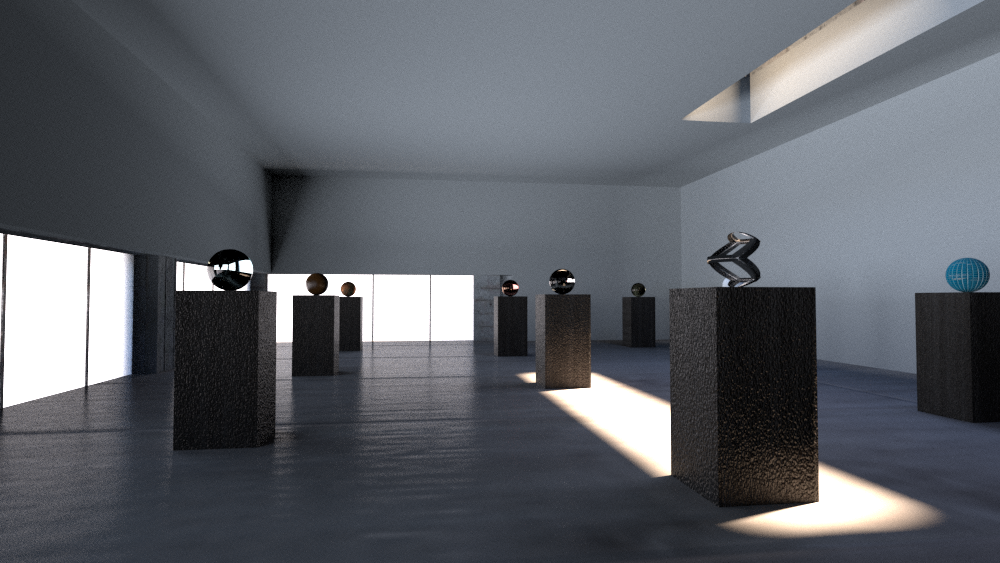
\includegraphics[width=\textwidth]{Images/Evaluation/BlackPavilion/PavPretoExample116x7204.png}
	\caption[Black Pavilion: Representation of the arts exhibition space with a skylight]{Black Pavilion: Representation of the arts exhibition space with the skylight in the top right corner.}
	\label{fig:blackpavilion}
\end{figure}

To this end, we conceived an algorithmic description of the building using the Khepri \ac{AD} tool and we used the Radiance lighting analysis tool to measure the \ac{sUDI} corresponding to different designs. Regarding the optimization, we decided to measure the performance of $10$ \acp{MOOA} regarding several indicators. Similarly to the previous case study, we aim at providing an average prediction of the behavior of each algorithm in this specific problem. As a result, we derived the combined Pareto fronts for each run and used them to compare the different algorithms. Each run comprises $200$ function evaluations, each of which takes on average $13.33$ minutes on dual \textit{Intel Xeon CPU E5-2670 @ 2.60GHz, 64GB RAM}.

Among the available algorithms and due to time constraints, we have selected $4$ metaheuristics, due to their acknowledged performance in other engineering applications: two evolutionary, $SPEA2$ and $NSGA$-$II$, and two particle-swarm, $SMPSO$ and $OMOPSO$. Additionally, we tested $6$ model-based algorithms, including $RF$+$Random$, $RF$+$NSGA$-$II$, $RF$+$SPEA2$, $GPR$+$Random$, $GPR$+$NSGA$-$II$, and $GPR$+$SPEA2$. \Cref{table:blackpavilion} shows the mean results of each algorithm for each of the evaluated unary indicators. 

\begin{table}[htbp]
	\centering
	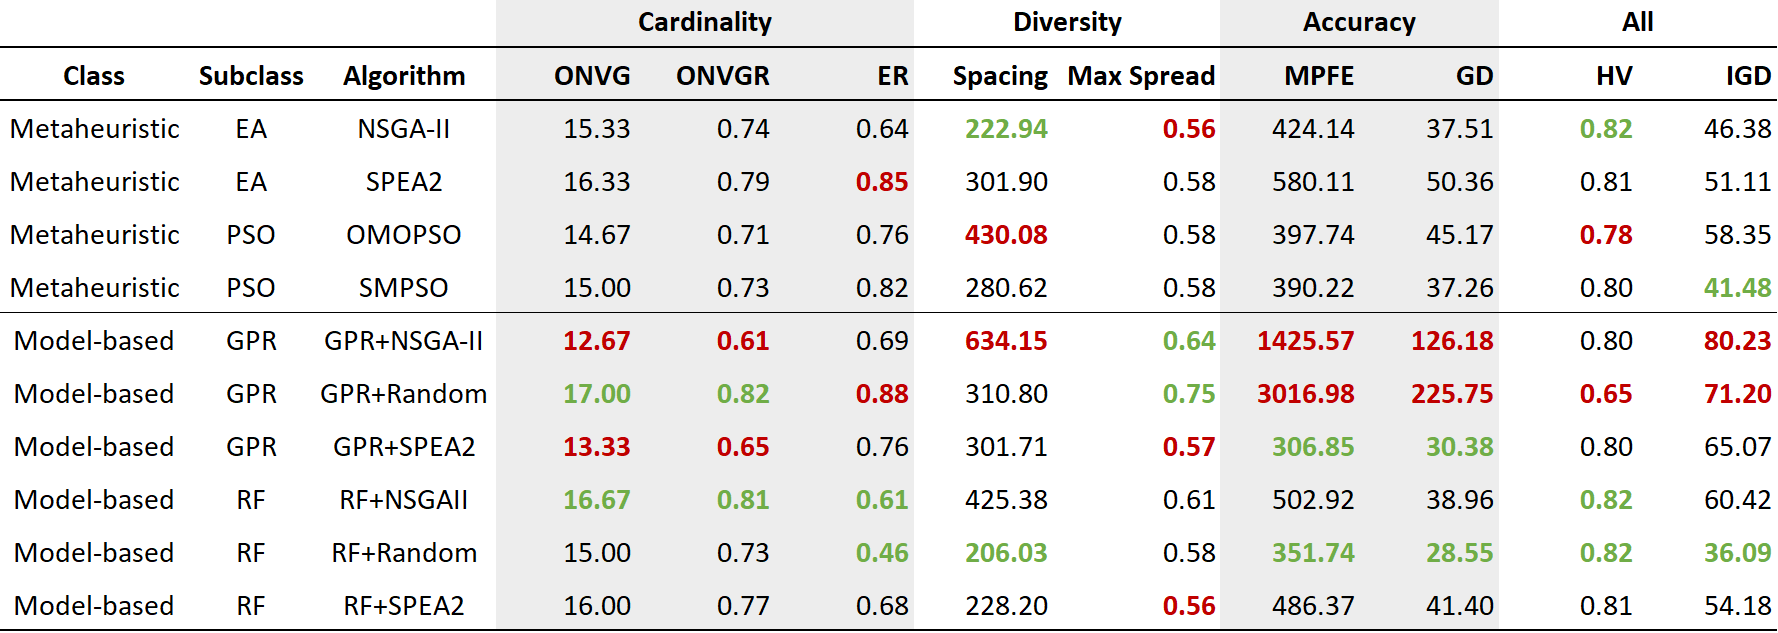
\includegraphics[width=\textwidth]{Images/Evaluation/BlackPavilion/Results_Mean_20190416.PNG}
	\caption[Black Pavilion: Mean performance values of the algorithms' results]{Black Pavilion: Comparison of the algorithms' results for the bi-objective black pavilion optimization problem. Results are averaged over $3$ runs, each with $200$ evaluations.}
	\label{table:blackpavilion}
\end{table}

Firstly, regarding the cardinality aspect of the results, $GPR$+$Random$ and $RF$+$NSGA$-$II$ attained, on average, more solutions, whereas $GPR$+$NSGA$-$II$ and $GPR$+$SPEA2$ obtained fewer solutions. Note, however, that although $GPR$+$Random$ retrieved the mean highest number of solutions, this value is subject to large variations (as evidenced in \cref{table:blackpavilionstd}) and, in fact, when examining the results per run, $GPR$+$Random$ retrieved $13$, $14$, and $24$ solutions. Regarding metaheuristic algorithms, evolutionary-based algorithms have achieved relatively higher cardinalities than the \ac{PSO}-based ones. 

Notwithstanding the cardinality of the retrieved Pareto fronts, it is important to determine how many of these solutions actually lie in the combined Pareto front, which is measured by the \ac{ER} indicator. In this case, $RF$+$Random$ presents an \ac{ER} value less than $0.5$, which means that, on average, more than half of the retrieved solutions lie in the combined Pareto front. The second and third best performing algorithms were $RF$+$NSGA$-$II$ and $NSGA$-$II$ with values of $0.61$ and $0.64$, respectively. Conversely, $SPEA2$ and $GPR$+$Random$ presented the worst \ac{ER} values. Interestingly, even though $GPR$+$Random$ returned on average more solutions than all other algorithms, it barely succeeds in retrieving one optimal solution lying in the combined Pareto Front.

Secondly, when considering the dispersion of the solutions found by the algorithms in the objective space, $RF$+$Random$ and $NSGA$-$II$ exhibit the first and second best results. On the other hand, $GPR$+$NSGA$-$II$ presents the mean worst Spacing value, hence suggesting that the solutions retrieved by this algorithm are not evenly spread across the objective space. While $OMOPSO$ presents the mean second worse performance in terms of the Spacing indicator, this result is associated to a large deviation, which derives from the fact that in the third run the algorithm was able to retrieve a more uniform distribution (see \cref{sec:blackpavilionextra}). Interestingly, $RF$+$NSGA$-$II$, presenting the third worse Spacing value, also presents a large standard deviation. Upon a careful review over this algorithm's Pareto fronts for each run, this variation is explained due to a single solution in the second run that is offly distant from all others, which highly influences the results. 

When considering the maximum extent of the Pareto fronts discovered by each algorithm, i.e., the Maximum Spread (named Max Spread in \cref{table:blackpavilion,table:blackpavilionstd}), $GPR$+$Random$ and $GPR$+$NSGA$-$II$ are the most performing algorithms, having achieved values of $0.64$ and $0.75$, respectively. Conversely, the other \ac{GPR}-based algorithm, $GPR$+$SPEA2$ achieved the second worse performance with a value of $0.57$, only surpassing the performance of $NSGA$-$II$ and $RF$+$SPEA2$, whose value was $0.56$. 

Thirdly, we measured the mean accuracy of the Pareto fronts retrieved by each algorithm. In terms of the \ac{MPFE} indicator, $GPR$+$SPEA2$ deviates the least from the combined Pareto front, with a value of $306.85$ for the furthest solution. The second best algorithm is also a model-based algorithm, $RF$+$Random$, whose furthest found solution lies on average within $351.74$ from the combined Pareto front. The third and fourth best performing algorithms were \ac{PSO}-based algorithms, which achieved close to optimal solutions as well. Conversely, $GPR$+$NSGA$-$II$ and $GPR$+$Random$ achieved the worst results in terms of \ac{MPFE}, identifying nondominated solutions at a distance of $1425.57$ and $3016.98$ from the closest solution in the corresponding combined Pareto fronts. A noteworthy observation is that while the worse performance of $GPR+Random$ results mainly from its poorer performance during the second run (see \cref{sec:blackpavilionextra}), the same does not happen with $GPR$+$NSGA$-$II$, whose \ac{MPFE} results for the first and third run remain approximately on $1600$. 

\begin{table}[htbp]
	\centering
	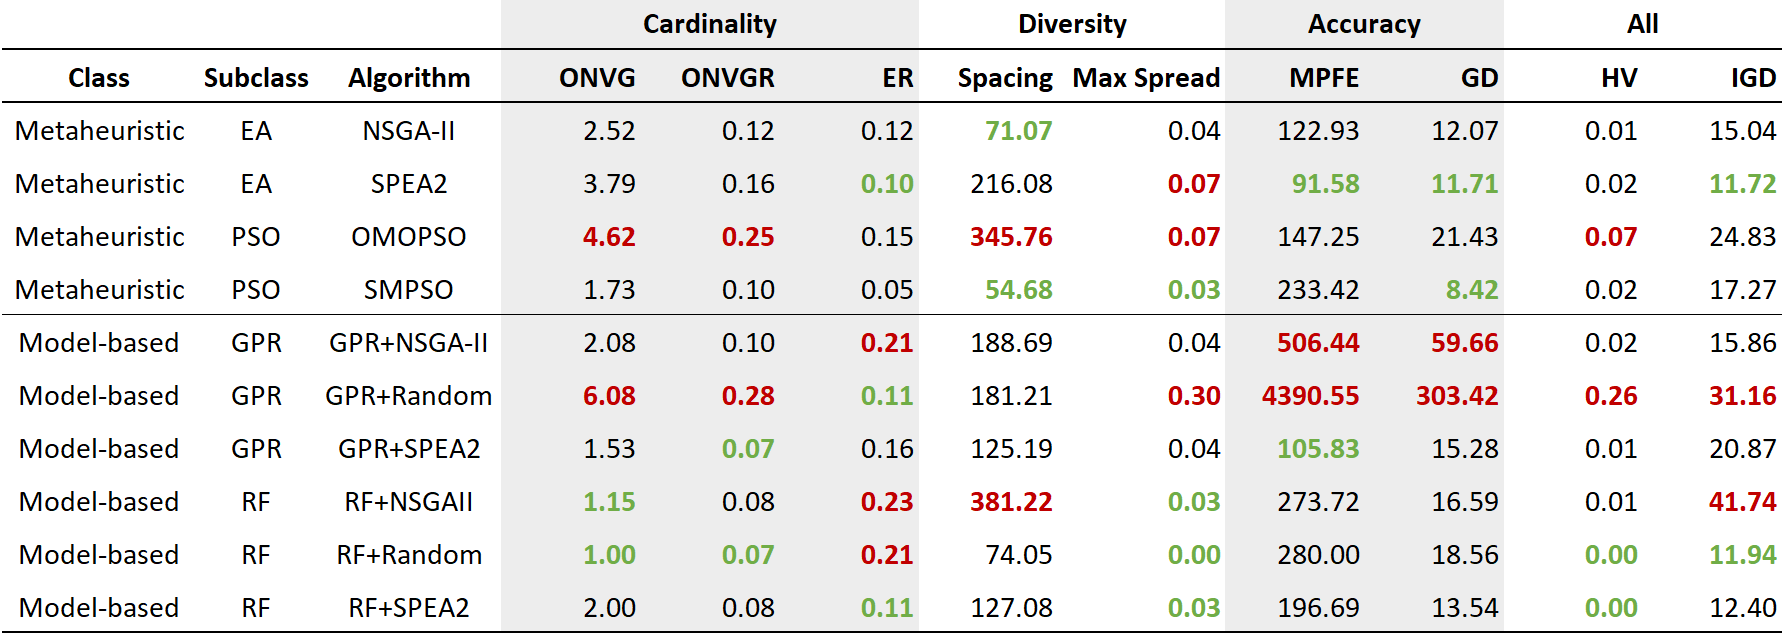
\includegraphics[width=\textwidth]{Images/Evaluation/BlackPavilion/Results_Std_20190416.PNG}
	\caption[Black Pavilion: Standard deviations of the performance indicators results, discriminated by each algorithm]{Black Pavilion: Standard deviation values for the performance indicators, discriminated by algorithm. Results are averaged over $3$ runs, each with $200$ evaluations.}
	\label{table:blackpavilionstd}
\end{table}

In addition to \ac{MPFE}, we measured the \ac{GD} of each Pareto front. Although the results for this metric resemble the ones obtained with \ac{MPFE}, there are a few differences, namely, in terms of the best performing algorithm. In this case, $RF$+$Random$ is the best algorithm, followed closely by another model-based algorithm, the $GPR+SPEA2$. The third and fourth best results correspond to two metaheuristic algorithms, namely, $NSGA$-$II$ and $OMOPSO$, respectively. Other model-based algorithms, like $RF$+$NSGA$-$II$ and $RF$+$SPEA2$ exhibit the fifth and sixth best performance. The two worse algorithms are $GPR$+$NSGA$-$II$ and $GPR$+$Random$. Note, however, that $GPR$+$Random$'s high variance is, once again, mainly due to its poorer performance on the second run. Conversely, the results obtained by $GPR$+$NSGA$-$II$ are relatively distant in the first and third runs (see \cref{sec:blackpavilionextra}).

Finally, we used \ac{HV} and \ac{IGD} to circumvent some of the limitations inherent to other performance indicators, namely, the fact that other indicators exclusively rely on a unique aspect. Contrastingly, \ac{HV} and \ac{IGD} provide a measure of all three aspects. Regarding the \ac{HV}, three algorithms achieved the best result, including a metaheuristic, $NSGA$-$II$, and two model-based algorithms, $RF$+$NSGA$-$II$ and $RF$+$Random$. By observing the \ac{HV} column in \cref{table:blackpavilion}, it is possible to observe that all algorithms with the exception of $OMOPSO$ and $GPR$+$Random$ achieved similar results of \ac{HV}. Once more, the poor performance of $GPR$+$Random$ and $OMOPSO$ during the second run severely hindered their average performance.

The analysis of the \ac{IGD} indicator revealed that the $RF$+$Random$ was the best algorithm. Surprisingly, the second, third, and fourth best algorithms belong to the metaheuristic class, namely, $SMPSO$, $NSGA$-$II$, and $SPEA2$. These results can be explained by the overall spread of the associated Pareto fronts over the objective space covered by the combined Pareto front, as well as with a more uniform distribution across the objective space. In other words, while $SPEA2$ yields a reasonable number of optimal solutions, each covering regions close to the Pareto solutions' clusters in the combined Pareto front, $GPR$+$SPEA2$ yields a lower number of optimal solutions that fail to cover the different optimal regions identified in the combined Pareto front. Therefore, its \ac{IGD} value will be inherently lower, as \ac{IGD} measures how close the combined Pareto front is to the Pareto fronts identified by each algorithm. When considering the worst algorithms, $GPR$+$NSGA$-$II$ presented the worst performance, followed by $GPR$+$Random$. Their lower performance resulted from the poor distribution of optimal solutions in the objective space, as well as from their generalized inability to discover solutions belonging to the combined Pareto front. 

\begin{figure}[htbp]
	\centering
	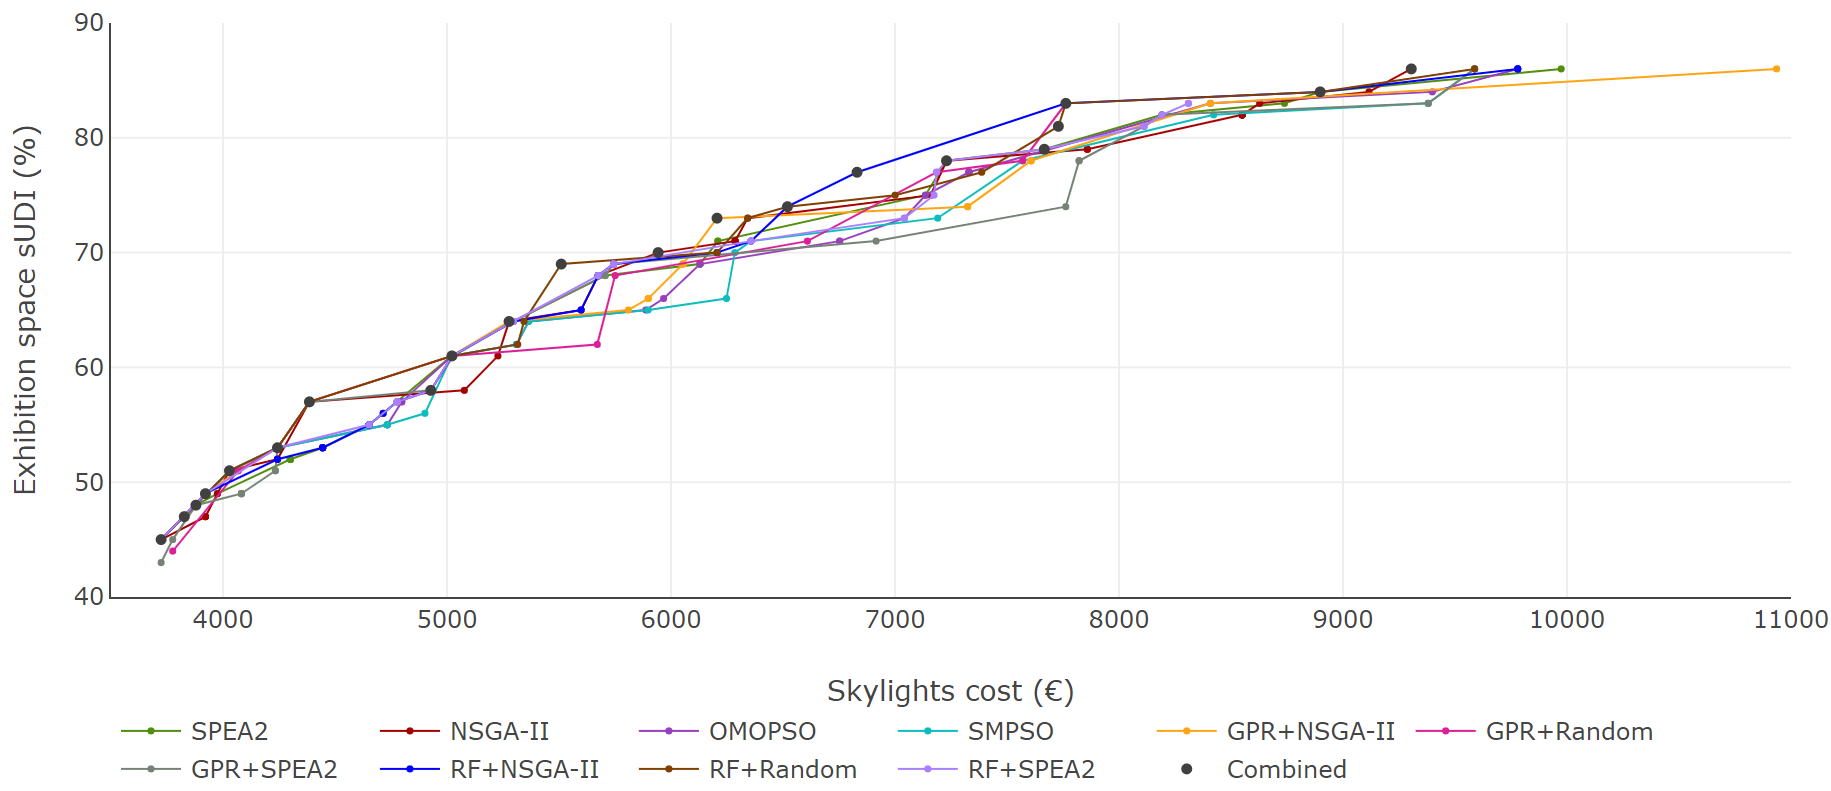
\includegraphics[width=\textwidth]{Images/Evaluation/BlackPavilion/All_Algorithms_all_runs-2019-04-16.png}
	\caption[Black Pavilion: Pareto front plot]{Black Pavilion: Line plot of the Pareto fronts retrieved by each algorithm measuring the daylight conditions of the exhibition space in function of the skylights cost. These fronts are obtained by combining the values of the $3$ runs for each algorithm. The combined Pareto front is formed by finding the nondominated solutions from all the evaluated solutions.}
	\label{fig:blackpavilionallruns}
\end{figure}

\Cref{fig:blackpavilionallruns} presents the overall performance of all the tested algorithms after combining the results of the $3$ runs. We can observe that in general, all algorithms converged towards the combined Pareto front, represented by the black points. Moreover, it is possible to observe that, overall, $RF+Random$, $RF+NSGA$-$II$, and $NSGA$-$II$ converged towards the combined Pareto front with only a few solutions missing the combined Pareto front. On the other hand, algorithms, like $SPEA2$, $SMPSO$, and $GPR+Random$ partially converged to the combined Pareto front, however, for values of cost above $5500$€ these algorithms begin to deviate from the combined Pareto front.

\subsection{Final Remarks}

In this chapter, we have studied the application of different optimization algorithms to three \ac{BPO} case studies. To that end, we have applied the optimization methodology described in \cref{chap:implement}, which uses the Khepri \ac{AD} tool and the optimization framework discussed in \cref{chap:architecture}. We have also used the analytical tools Radiance and Robot to measure the daylight and structural aspects of the different designs generated during the optimization.

The first case study belongs to an unconstrained \ac{SOO} problem, which involved the optimization of the daylight performance of a private house. We tackled this problem in two different ways. On the first stage, we followed a simple design of experiments approach, where we applied two sampling algorithms. On the second stage, we followed an \ac{SOO} approach, for which we have tested $13$ \acp{SOO} derivative-free algorithms, including $5$ direct-search, $5$ model-based, and $3$ metaheuristics. Results showed that, on average, global model-based algorithms exhibit best performance both in earlier and final stages of the optimization process. The same does not happen with metaheuristics that, although exhibiting a reasonable performance in earlier stages of the design, even surpassing the performance of global direct-search algorithms, stagnate shortly after. Conversely, global direct-search algorithms performed reasonably well, excelling metaheuristics shortly after $20$ evaluations. Moreover, we proved that both local direct-search and model-based algorithms can be fast solvers, when provided with reasonable initial solutions. Indeed, two local algorithms converged towards optimal solutions after just $8$ evaluations. Given that each function evaluation took approximately $7$ minutes to complete, this evaluation difference becomes crucial for more complex optimization processes.

The second case study comprises an unconstrained bi-objective optimization problem of an arc-shaped space frame, whose objectives were the structural and the aesthetic aspects of the space frame. To that end, we evaluated the performance of $19$ \acp{MOOA}, $10$ metaheuristics, and $9$ model-based. Given the higher dimensionality of the algorithms' results, we measured the algorithms' performance in terms of the cardinality, diversity, and convergence of the retrieved results. The difficulties underlying \acp{MOOA} quality measurements prevailed during this case study. To circumvent this limitation, we evaluated the algorithms performance through a combination of \ac{MOO} indicators (see \cref{ssec:performance}) and line plots of the Pareto fronts returned by each algorithm. The results showed that \ac{PSO}-based metaheuristics algorithms achieved the overall best performance, whereas \ac{ES}-based metaheuristics algorithms achieved the overall worst performance. Moreover, while model-based algorithms did not outperform any of the metaheuristics algorithms, results suggest that model-based algorithms exploiting \ac{PSO} search strategy outperform other model-based variants, involving $NSGA$-$II$ or $Random$ strategies. Additionally, model-based algorithms depending on $Random$ search strategies seem to perform worse than other variants. 

The third and final case study also comprised an unconstrained bi-objective optimization of the cost and daylight aspects of an art exhibition space. To that end, we tested $10$ \acp{MOOA}, $4$ metaheuristics and $6$ model-based. Similarly to the previous case study, we also used a combination of Pareto front line plots with a set of \ac{MOOA} performance indicators to measure the quality of the optimization results. Results show that, contrastingly to the previous problem, \ac{PSO}-based algorithms fell short in terms of performance. Instead, $RF+Random$, a model-based algorithm, was one of the top performing algorithms, followed by $NSGA$-$II$, a metaheuristic algorithm. 

In conclusion, a thorough analysis of the case studies evidences that there is no single class, subclass, or algorithm that outperforms all others. This corroborates the ideas of Wolpert's optimization \ac{NFLT}\cite{Wolpert1997NFLT}. In the first problem, although global model-based algorithms achieve better results when no information is known, direct-search local algorithms are also able to achieve close to optimal results in fewer iterations. Moreover, while we did not test direct-search algorithms in a \ac{MOO} context problem, it is possible to visualize that even between each category of derivative-free algorithms, either metaheuristic or model-based, different subclasses present significantly different outcomes according to each problem's characteristics. For this reason, we conclude that prior to the selection of an optimization algorithm, users should test different algorithms for a fixed number of evaluations or a fixed amount of time. The proper algorithm selection can have beneficial impacts on the performance of an optimization process, namely in the time and quality of obtained results. In fact, not only do users select the most promising algorithm, but they can also explore the already evaluated solutions to hot-start local algorithms or to create an initial surrogate model. This surrogate model can be explored to either determine an approximated behavior of the objective function or to perform optimization. 

Another interesting conclusion is related to the impact of model-based algorithms in \ac{MOO} problems. Although model-based algorithms were not particularly successful in the second case study, they attained relatively better performance in the third case. More comparative \ac{MOO} studies are necessary, especially in \ac{BPO} problems, where studies combining model-based algorithms with Pareto-based optimization approaches are rare. In this vein, this dissertation contributes to bridge this gap and, in the next chapter, we outline future paths of research to further enrich these studies.

Finally, we conclude that there is no consensus regarding the best way to assess the quality of these algorithms and that this comparison should involve the computation of different \ac{MOO} indicators, the visualization of the Pareto front plots, and some critical thinking. 